
\section{Turbulent Boundary layers under adverse pressure gradients}

A wall-bounded flow can see pressure gradients as a result of the curvature of the wall, but also as a result of a change in the direction/velocity of the outer flow $(U_{e}, V_{e}, W_{e})$. Turbulence is already a complex problem in a ZPG case with the only parameter being the Reynolds number (momentum/viscous forces), if another parameter such as pressure gradients is added, the complexity of the problem increases and it becomes difficult to distinguish what phenomena is caused by the $\Rey$ effects or by the PG history of the flow.
In order to properly study APG TBLs, first we should try to define a canonical simple case, that is a well-defined APG along the streamwise development of the TBL, this is what we refere as the PG history of the flow.
To address this problem, different pressure-gradient parameters have been defined in literature, such as the Rotta-Clauser PG parameter $\beta$, or a general $\Lambda_{inc}$ which in \cite{Gibis2019} is studied with different length and velocity scales.
In our simulations of moderate APGs we have used $\beta$ defined as
\begin{equation}
    \beta(x) = \frac{\delta^*}{\tau_w} \pdv{P}{x},
\end{equation}
where $\pdv{P}{x}$ is the averaged pressure-gradient, $\tau_w$ is the shear stress at the wall, and $\delta^*$ is the displacement thickness, which for an incompressible flow is defined as
\begin{equation}
    U_e \delta^* = \int_{0}^{\delta_{99}} (U_e - U) dy
\end{equation}

% IDEA behind beta
The idea behind the $\beta$ parameter is to stablish an integral equilibrium of forces across the TBL, in this way, every section of the TBL is subjected to the same dimensionless state of forces.
To clear this idea, Fig.~\ref{fig:scheme_beta} shows a scheme of a section of the BL, where the main forces are due to the streamwise pressure-gradient and the stress at the wall.

\begin{figure}
    \centering
    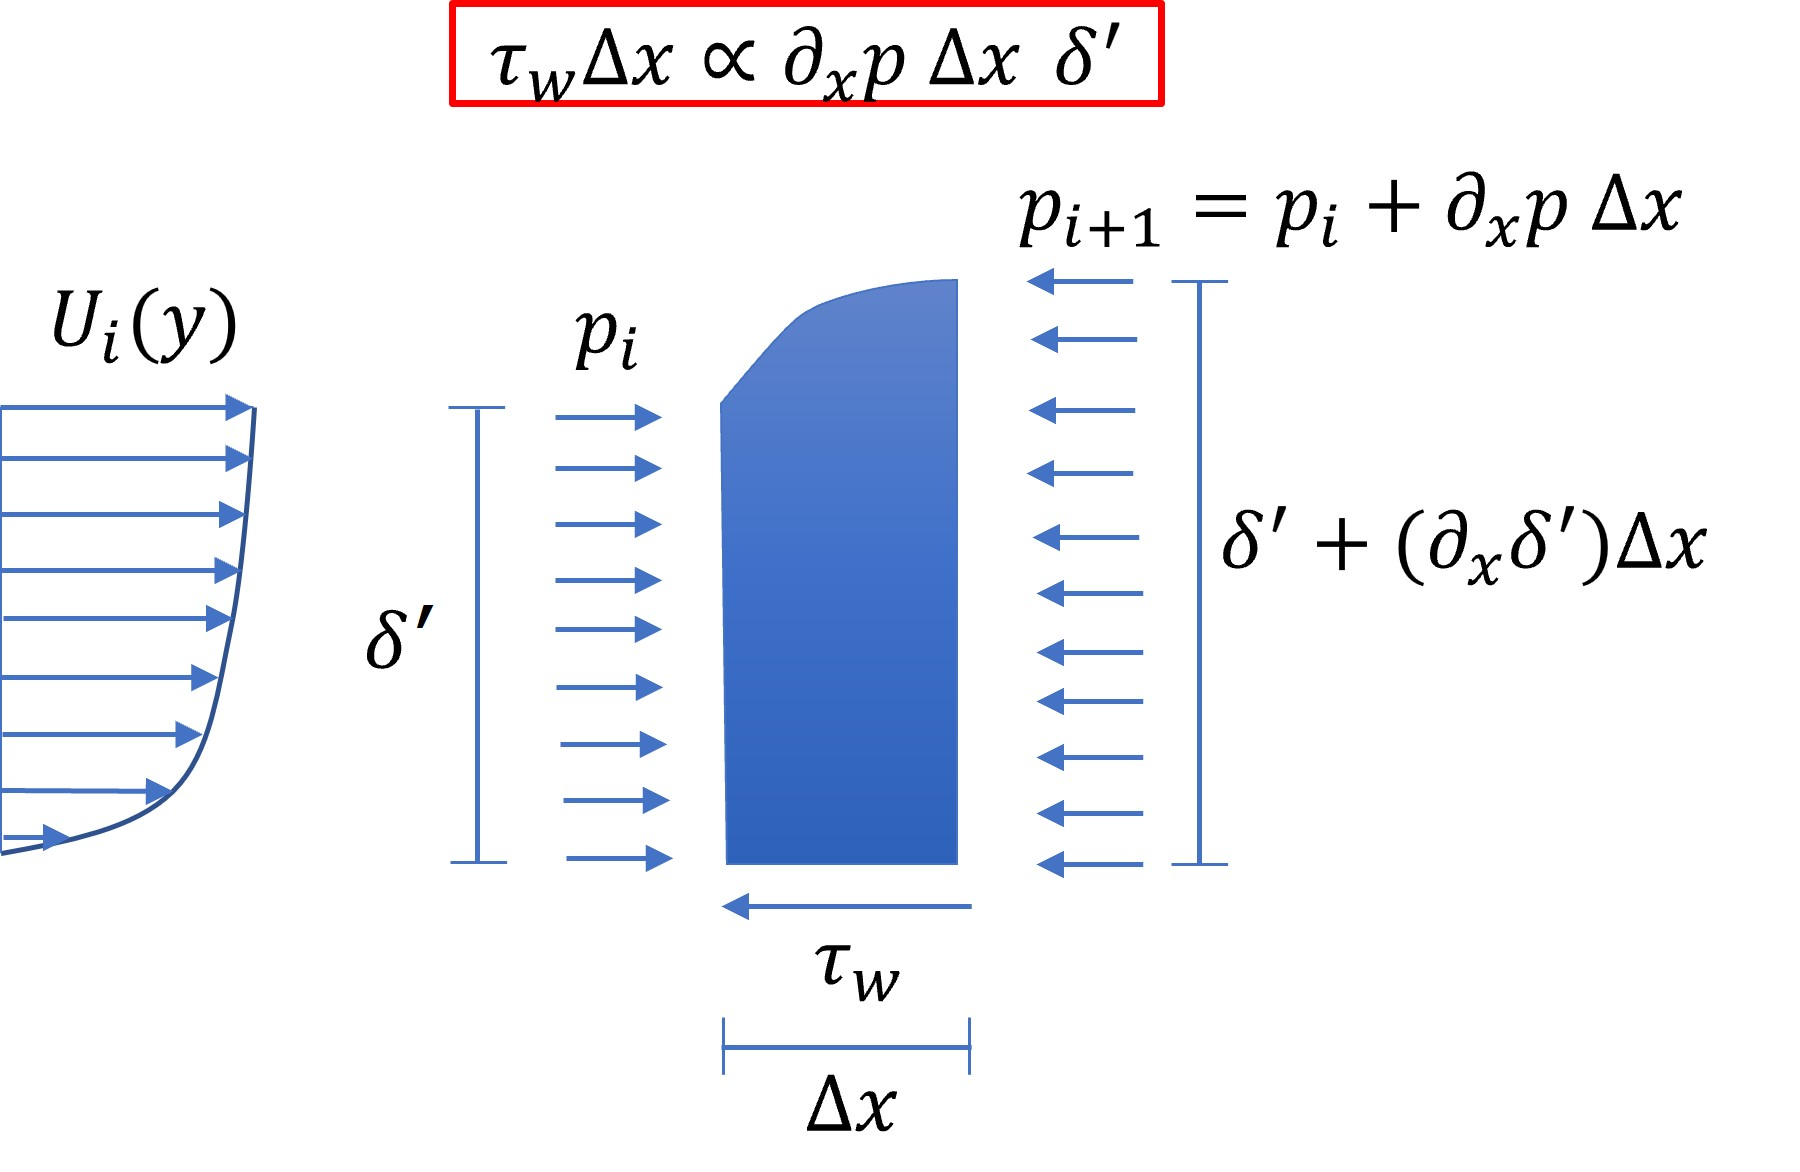
\includegraphics[width=0.90\textwidth]{imgs/schemes/scheme_beta.jpg}
    \caption{Stresses around a section of a BL.}
    \label{fig:scheme_beta}
\end{figure}

Integrating the streamwise momentum equation over the wall-normal direction, under several assumptions, it is possible to obtain an equation which relates the integral parameters $\delta^*$, $\theta$ and $\beta$, therefore, from an integral approach, the thickness $\delta \myprime$ is chosen equal to $\delta^*$. 



\section{Statistics}
In \textbf{Paper 1} we explore the statistical quantities of TBLs under APGs. The novelty respect to the available literature was in the high fidelity database used for the ZPG and APG TBLs. Both simulations show the development of the TBL from low Reynolds numbers such as those of previous numerical databases, and reach large Reynolds numbers such as those obtained in experiments. This characteristic works as a bridge to validate previous simulations as well as the current simulations, since they have been compared successfully with experimental data.
A benefit of numerical experiments is that the amount of quantities measured are larger than in experimental databases. This allows to have better measurements close to the wall and obtain decomposition such as spanwise spectra.

In Fig.~\ref{fig:U_uu_cap2}(a) we show the inner scaled $U$ and $\sqrt{\overline{u\myprime u\myprime}}$ for a $\Rey_{\tau}=500$, where the low Reynolds number simulations are already fully developed, while the experimental database does not have measurements. A higher $\Rey_{\tau}=2000$ is required by the experiments to have a fully developed near-equilibrium APG, and the LES ZPG and the new b1.4 simulation are able to achieve those Reynolds numbers.
The experimental data and b1.4 are in a similar range of $\beta$ and their statistics show a good agreement in the streamwise components.
The effects of the APG in $U$ show a lower $U^+$ for larger $\beta$ in the logarithmic region, and a larger effect in the wake region. At higher Reynolds numbers, the logarithmic region enlarges and the near-equilibrium APG and the ZPG profiles get closer.
In the turbulent perturbations, the near-wall or inner peak of $\sqrt{\overline{u\myprime u\myprime}}^+_{IP}$ grows in value with both the Reynolds number and the APG effects and its wall-normal position $y_{IP}^+$ seems to slightly increase with both APG and $\Rey$ effects. In \cite{Pozuelo_JFM_22} this trend is shown, where a filter was used to avoid saw-tooth jumps due to the wall-normal resolution close to the wall.
Larger Reynolds numbers allows for larger scales to live in the logarithmic/wake region and for a separation of the scales to be seen. This is first seen as lower decay in $\sqrt{\overline{u\myprime u\myprime}}$ in the ZPG in the logarithmic/wake region and a development of an outer peak for APG profiles. Larger $\beta$ increase the value of the outer peak of $\sqrt{\overline{u\myprime u\myprime}}$. The trends for the outer peak value and wall-normal position of the RS,  $\overline{u\myprime u\myprime}_{OP}$ and $y_{OP}$ where analysed in \cite{Pozuelo_JFM_22}. 


\begin{figure}
    \centering
    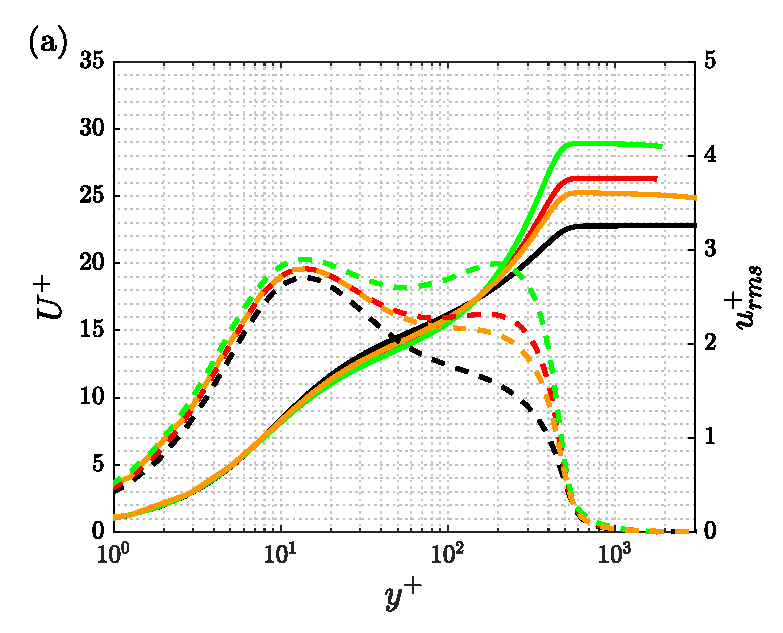
\includegraphics[width=0.49\textwidth]{imgs/stats/U_uu_a.eps}
    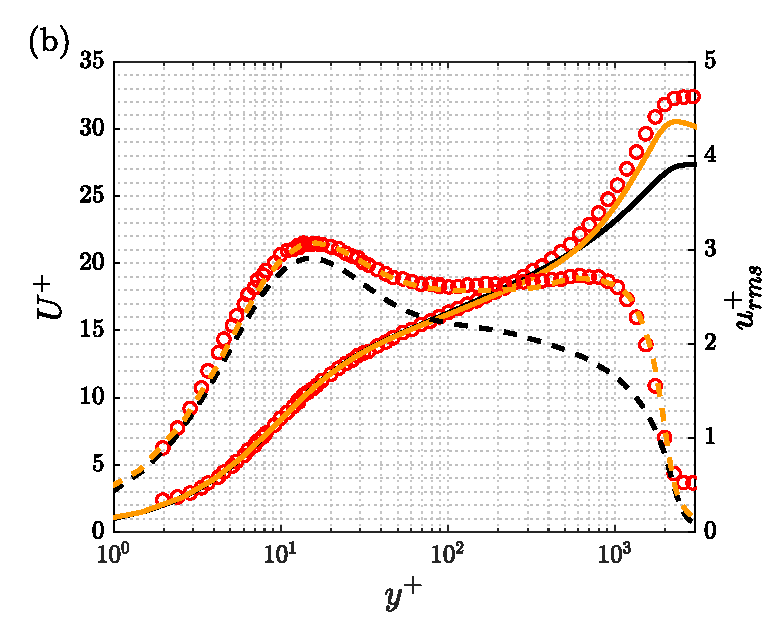
\includegraphics[width=0.49\textwidth]{imgs/stats/U_uu_b.eps}
    \caption{Mean streamwise $U$ (solid lines) and streamwise root mean square $u_{rms}$ or strandard deviation of the streamwise velocity (dashed lines). Wall-normal profiles taken at: (a) $\Rey_{\tau}=500$, (b) $\Rey_{\tau}=2100$. }
    \label{fig:U_uu_cap2}
\end{figure}

\subsection{Cf}

\subsection{RS}


\subsection{Spectral decomposition}
To have a better understanding on the perturbations we can use some mathematical tools such as the decomposition of the spatial-temporal signal using correlations, orthogonal modes, coherent structures, etc.
The use of orthogonal modes allows to decompose the energy of the perturbations into each mode in an unique way, so the sum of the energy contained in all the modes is equivalent to the total energy of the perturbations. 

In signal analysis an orthogonal decomposition which is commonly used is the Fourier decomposition which enables to look for phenomena that repeats with a certain time or spatial frequency. The energy or power associated with each mode is called energy spectra (if the signal is finite such as pulses) or power spectra (if the signal is such as sinusoidal waves, whose domain and energy is not finite, however its power is). Remember that the power is the ratio of the energy over time, where the time goes to infinity (in the case of using temporal series).
Since we are dealing with signals which are periodic in the homogeneous dimension $z$ and are not limited in time, we will use the terminology of power spectra (PS) instead of energy spectra. 
The modes in $z$ have a wavenumber $k_z$ and a wavelength $\lambda_z=2\pi/L_z$ where $L_z$ is the spanwise period of the domain. The same analysis can be applied in time, where we will use $k_t$ and $\lambda_t$.
For a signal $x(t)$, with $X(k_t)$ being its Fourier transform, the power of each mode is $|X(k_z)|^2$, the squared amplitude of the mode. For a perturbation velocity, the power can be calculated as,
\begin{equation}
    PS_{u_i\myprime u_j\myprime}(k_z) = \mathcal{F}(u_i \myprime)  \mathcal{F}^*(u_j \myprime),
    \label{eq:power_sp}
\end{equation}
where $\mathcal{F}()$ is the Fourier transform and $\mathcal{F}^*()$ represents the complex conjugate and the definition has been expanded to include the power spectra of the quantity $\langle u_i\myprime u_j\myprime \rangle_{z}$, also known as cospectra.
Using the properties of the Fourier transform, the multiplication in Fourier space represented in Eq.~\ref{eq:power_sp} represents the Fourier transform of the two-point correlation function $\mathcal{R}_{u_i\myprime, u_j\myprime}(\delta z)=u_i\myprime \star u_j\myprime$, where $\delta z$ is the lag or distance between the two points where we look for the correlation of their velocity perturbations. According to the Wiener--Khinchin theorem, we can calculate the PS through as the Fourier transform of $\mathcal{R}_{u_i\myprime, u_j\myprime}$ or from the power spectra throught the inverse Fourier transform $\mathcal{F}^{-1}()$ we can obtain the two-point correlation function.

Note that for velocity perturbations, since Fourier modes are orthogonal, the sum of the PS for all the modes is equal to the averaged Reynolds stress,
\begin{equation}
    \langle u_i\myprime u_j\myprime \rangle_{z} = \sum_{k_z} PS_{u_i\myprime u_j\myprime}(k_z)
\end{equation}

This step can be performed for each time step and averaged over time to obtain $\langle\langle u_i\myprime u_j\myprime \rangle_{z}\rangle_{t} = \overline{u_i\myprime u_j\myprime}$ or it can also be the result of a 2D spectral decomposition in both time and $z$, where the sum extends to all the spatial and temporal modes.

The PS is useful for discrete systems, and it is the first step when we calculate numerically the spectra of a the Reynolds-stresses. It is also interesting to see how the power spectra is distributed along the wavenumbers or the wavelengths, obtaining a power spectral density (PSD).
The average in time of the PSD in wavenumbers is $\phi_{u_i\myprime u_j\myprime}=\langle PS \rangle_t/\mathrm{d} k_z$ while the average in time PSD in wavelengths is $\psi_{u_i\myprime u_j\myprime}= \langle PS \rangle_t/\mathrm{d} \lambda_z$. Both densities can be linked using $\mathrm{d}(\lambda_z) = \mathrm{d}(2\pi/k_z) = -2\pi\mathrm{d}k_z/k_z^2$:

\begin{equation}
    \psi_{u_i\myprime u_j\myprime} = 
    \frac{ \langle PS_{u_i\myprime u_j\myprime} \rangle_t}{\mathrm{d} \lambda_z} =
    -\frac{ \langle PS_{u_i\myprime u_j\myprime} \rangle_t}{\mathrm{d} k_z} \frac{k_z^2}{2\pi},
\end{equation}
where the minus sign is taking care by inverting the limits of integration to obtain the total RS (small to large wavenumbers is equivalent to integrate from large to small wavelengths).

\begin{equation}
\label{eq:sum_ps}
    \overline{u_i\myprime u_j\myprime} = 
    \int_{k_z=k_0}^{k_z=k_{N}}   \phi_{u_i\myprime u_j\myprime}  ~ \mathrm{d} k_z =
    \int^{\lambda_z = 2\pi/k_0}_{\lambda_z = 2\pi/k_{N}}  \psi_{u_i\myprime u_j\myprime}  ~ \mathrm{d} \lambda_z
\end{equation}

In Fig.~\ref{fig:PS_PSD} we show for a ZPG TBL, different representations of the PSD of $\overline{u\myprime u\myprime}$ where the image with the black contours represent a streamwise profile at $\Rey_{\tau}=2000$ while the red contours are taken at a position where $\Rey_{\tau}=500$.

\begin{figure}[h!]
\centering
% \captionsetup{width=0.99 \textwidth}
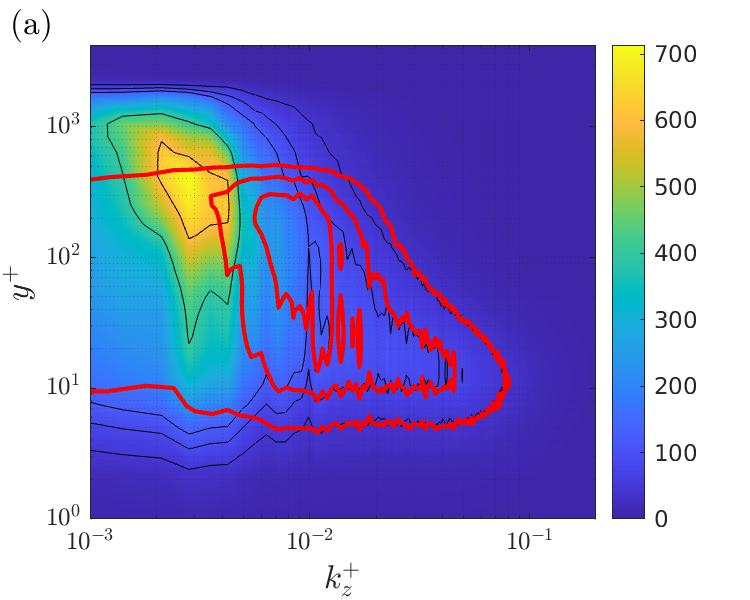
\includegraphics[width=0.32\textwidth ]{imgs/spec/ZPG_Ret_500_2000_PSdkz_kz_ltau_y_ltau.jpg}
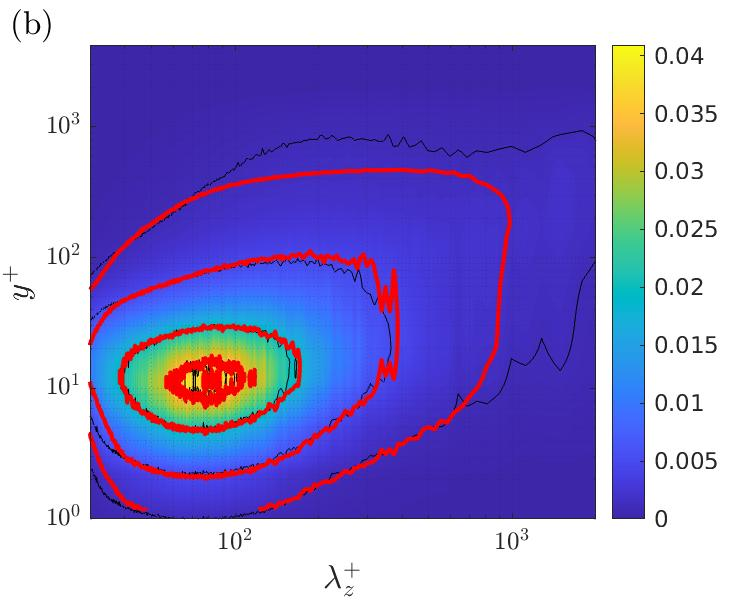
\includegraphics[width=0.32\textwidth]{imgs/spec/ZPG_Ret_500_2000_PSdlambdaz_lambdaz_ltau_y_ltau.jpg}
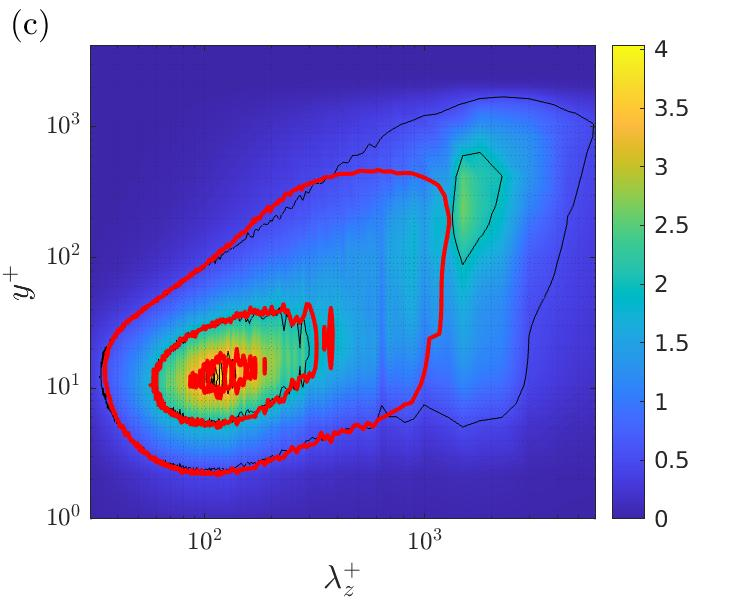
\includegraphics[width=0.32\textwidth]{imgs/spec/ZPG_Ret_500_2000_kPSdkz_lambdaz_ltau_y_ltau.jpg}
\caption{ \label{fig:PS_PSD} Spanwise spectra of the streamwise Reynolds stress $\overline{uu}(y)$. (a) Power spectral density $\phi_{u\myprime u\myprime}(y,k_z)$; (b) Power spectral density $\psi_{u\myprime u\myprime}(y,\lambda_z)$; (c) premultiplied power spectral density $k_z\phi_{u\myprime u\myprime}$. Wavenumbers, wavelengths, wall-normal position and power spectra scaled in viscous units.}
\end{figure}
% contours: Retau 2000: [40 80  120 400 600]; [0.001 0.005 0.02 0.035 0.04] ;  [ 0.5 2 3.5]; 
% contours: Retau  500: [40 80  120        ]; [0.001 0.005 0.02 0.035 0.04] ;  [ 0.5 2 3.5]; 

The PS and the PSD in the wavenumbers $\phi_{u\myprime u\myprime}(y,k_z)$ present the same features as in Fig.~\ref{fig:PS_PSD}(a), since $dk_z$ or $dk_z^+$ are constant factors that does not vary with the wavenumbers. It shows a high content of power/energy of structures with a very low wavenumber which are very wide. It is possible to see similarities in the contours at different Reynolds numbers (red and black lines) in the region of high wavenumbers (small scales), although the energetic level is very low compared to that of the low wavenumbers (large scales).
The PSD in wavelengths $\phi_{u\myprime u\myprime}(y,\lambda_z)$ is represented in Fig.~\ref{fig:PS_PSD}(b) and it focuses on the small scales. It shows that the density of power/energy in the small scales (short wavelengths) is very similar at different Reynolds numbers and larger than the PSD of the wider scales (large $\lambda_z^+$). 
From Fig.~\ref{fig:PS_PSD}(a) and (b) we see that the small scales have a small content of the total RS energy, but their small size make the density in waveleghts to be very concentrated, while for the wider scales is the opposite, the energy they contain is very large, but their big size make the PSD to be very low or disperse.
If we write both PSD as a function of $\phi_{u\myprime u\myprime}$, in Fig.~\ref{fig:PS_PSD}(a) we show $\phi_{u\myprime u\myprime}$ while in Fig.~\ref{fig:PS_PSD}(b) it would be $k_z^2 \phi_{u\myprime u\myprime}$, the premultiplication factor $k_z^2$ is responsible to augment the effects of the small scales while diminishing the effects of the large scales. Fig.~\ref{fig:PS_PSD}(c) shows $k_z \phi_{u\myprime u\myprime}$, whose effect equilibrates the effect of the large and small scales obtaining a better visualization of both scales.

The premultiplied PSD $k_z \phi_{u\myprime u\myprime}$ is widely used and it has a geometrical explanation.
Since the range of energetic scales is so large that we observe very small scales close to the wall and very large scales of the size of $\delta_99$, the use of logarithmic axis helps to expand the region of small $\lambda_z$ and the region close to the wall.
If we use logarithms in the definition of wavelength, $ \mathrm{ln}(\lambda_s) = \mathrm{ln}(2\pi) - \mathrm{ln}(k_z)$, and apply the differential, $\mathrm{d}(\mathrm{ln} \lambda_z) = -\mathrm{d}(\mathrm{ln} k_z)$, and together with $\mathrm{d}k_z = k_z \mathrm{d}(\mathrm{ln} k_z)$ can be substituted in Eq.~\ref{eq:sum_ps} to obtain:
\begin{equation}
    \overline{u_i\myprime u_j\myprime} = 
    \int_{k_0}^{k_{N}}   \phi_{u_i\myprime u_j\myprime}  ~ \mathrm{d} k_z = 
    \int_{k_0}^{k_{N}}   \phi_{u_i\myprime u_j\myprime} k_z  ~ \mathrm{d}( \mathrm{ln} k_z) = 
    \int^{\lambda_0}_{\lambda_{N}}   \phi_{u_i\myprime u_j\myprime} k_z ~ \mathrm{d}( \mathrm{ln} \lambda_z).
\end{equation}

The premultiplication by $k_z$ can be seen here as a factor to visualize a corrected area after scaling the axis with a logarithmic scale.
From here on the PSD will always be represented in its premultiplied form $k_z\phi$ to have a clear visualization of the effects of large and small scales at the same time.

\subsubsection{Wide scales in turbulence. Channel Flows}
It has been seen that the big scales contains a large part of the turbulent energy, although the density spectral density is low.
When we model the turbulent flow, the size of the domain imposes a limit on the size of the scales that can be simulated. In a periodic domain, the largest scale corresponds to $L_x$ and the wider scale to $L_z$. Bigger scales will be seen as infinit in size because of the periodicity, and the spectral energy will be stored in the zero-wavenumbers.

The energy contained in the zero-wavenumbers is affected by the averaging.

If the size of the domain is not large or wide enough, the bigger turbulent scales will not be able to be captured and the energetic spectrum will not be correct, affecting the total statistics such as the Reynolds stresses and the mean velocity profiles.
Many analysis on the size of the domain has been performed on canonical turbulent channel flows for it simplicity.
\highlight{Minimal channels are those small domains that assure }
On the other way, the largest scales in channel flows where looked for in \highlight{CITAR ADRIAN que descubrieron bla bla}.
The study on the wider scales was based on two-point correlations, but no other study similar to \highlight{CITAR ADRIAN} was performed in the spanwise direction.

To have a better understunding of the wide scales obtained in APG TBLs and the effects of the domain size, we decided to study first the effect on wide-channels.
Three simulations were performed of turbulent channel flows at $\Rey_{\tau} = 550 $ under similar conditions, with the only excemption the width of their domains which was doubled from one channel to another as it can be seen in \highlight{Tabla de los channel}.
 


\subsubsection{Spectral results on APG}

In \textbf{Paper 1} the 1D spanwise spectra and the 2D spanwise and temporal spectra of the APG TBL where shown and compared to those of a ZPG TBL \citep{EAmorZPG}. By using percentage contours it was possible to show a similar behaviour in the mild APG and the ZPG simulations at different Reynolds numbers in the small-scale energy region close to the wall around an spectral near-wall peak or spectral inner peak (sIP) at $y^+\approx 15$ and $\lambda_z^+\approx 120$. Another region with similar shape is in the wake region with an spectral outer peak that seemed to scale with the Reynolds number.
Another region is that of small-scale energy in the wake region, which is only present in the APG simulation and not in the ZPG case.

\begin{itemize}
    \item show pcolor con APG y ZPG de uu, uv en Retau 500 y 2000
\end{itemize}

The spectra shows a similar region of small-scale energy close to the wall which is responsible of the near-wall peak the RS $\overline{u\myprime u\myprime}$. The effects of $\Rey$ and $\beta$ increase the value of $\overline{u\myprime u\myprime}_{IP}^+$, even if the most of the spectra is similar for APG and ZPG at different Reynolds numbers.
The outer-spectral peak in $k_z\phi_{uu}$ is also responsible of most of the energy contained in the ZPG in the wake region, and increasing $\beta$ it increases the energy to the point of growing the outer peak in $\overline{u\myprime u\myprime}_{OP}^+$. This behaviour is similar in the other components of the RS tensor, where at higher $\Rey$ numbers there are larger and energetic scales acting on the wake region and influencing all across the TBL.

\subsubsection{Scaling of APG spectrum}

In \textbf{Paper 2} we try to understand the trends of the inner and outer peaks in $\overline{u\myprime u\myprime}$ shown in \textbf{Paper 1}. Why the inner scaled inner-peak grows with the Reynolds numbers and with the APG effects. Is it still correct to use viscous scaling?. 
We perform a scaling analysis of the different energetic scales of the power spectral density for both ZPG and APG simulations and at different Reynolds numbers.
First we start from the features observed in $k_z\phi_{u\myprime u\myprime}$ which are an spectral near-wall/inner peak (sIP) and an spectral outer peak (sOP). The data is scanned to look for the maxima at a certain wall-normal position and the maxima at a certain frequency. Since $k_z\phi_{u\myprime u\myprime}$ is saved in a rectangular matrix, it is equivalent to obtain the maxima along columns and the maxima along rows.
At high Reynolds number the separation of scales even in ZPG TBLs, allows to distinguish clearly the presence of 2 maximal points for $\Rey_{\tau}>500$. Other techniques could be used to detect the local maxima, but this method was obtaining satisfactory results, specially the values of $f(y)=max(k_z\phi(k_z, y))_{k_z}$ since that function presents less noise and it is shown in \highlight{ Fig.~\ref{fig:scaling_OP} figura de los escalados de los picos} that once the Reynolds number is enough to have separation of scales, the outer peak clearly separates in the wall-normal direction from the spectral near-wall peak.
Once sIP and sOP are located in $k_z\phi(k_z, y)$, (usually we represent with $\lambda_z$), we try the inner and outer length scalings used in \textbf{Paper 1} to scale $\overline{u\myprime u\myprime}(y)$.
It is shown that the viscous length $\ell_{\tau}$ scales the size of the spanwise scales of the sIP $\lambda_{z, sIP}^+$ as well as the wall-normal position $y^+_{sIP}$.
The same method is used for the spectral outer peak. The outer scales $\delta^*$ and $\delta_{99}$ were used to scale independently the wall-normal location $y_{sOP}$ and the size of the scales $\lambda_{z, sOP}$.
In previous studies such as \cite{Kitsios2017} the $\delta^*$ scaling was successful for the $y_{OP}$ as well as for $y_{sOP}$ at much higher $\beta$, however, $\lambda_z$ was also scaled with the same scaling.
In \cite{tanarro_2020}, the outer scaling was performed with $\delta_{99}$ for both $y$ and $\lambda_z$, and the values of $\lambda_{z,sOP}$ were better collapsed than using $\delta^*$ as in \cite{Kitsios2017}.
Taking into account this previous studies, we allowed $y$ and $\lambda_z$ to have different length scalings, and found the optimal collapse of the region around the spectral outer peak using $y/\delta^*$ and $\lambda_z/\delta_{99}$.

Once we obtained the scalings for the wall-normal position and size of the scales for both sIP and sOP, we looked the region around those peaks using the respective scalings, obtaining a good collapse, however there was another region to investigate, which is the region of small-scale energy in the wake region.
Different scalings were tried for $\lambda_z$ looking to match the vertical part of the energetic contours of the APG simulation at different $\Rey$.
We observed that using $\lambda_z/\delta^*$, there is a collapse around $\lambda_z/\delta^*=0.3$. It could be argued that the scaling evolves gradually at different $\lambda_z$ up to the region around the sOP that clearly scale using $\lambda_z/\delta_{99}$.
To have a better idea of how big was the contribution of the small-scale energy in the wake region, but also to understand what is the influence of the large scales in the near-wall region, we tried to accumulate the energy from small to large scales for all the wall-normal positions. In a matrix containing the $PS(y,k_z)$, this is equivalent to do a cumulative sum $cumsum(PS(y,k_z))_{k_z}$ along $k_z$.
In \cite{EAmorZPG}, they limited a rectangular region around sIP, to probe that inner scaled energy in this region does not vary with the Reynolds number, but we have seen that there are different scalings at different heights of the TBL, therefore, the rectangular domain to integrate over $\lambda_z$ and $y$ may not be the optimal tool for this analysis.

With the idea of looking for the contribution of small and large scales using a cumulative sum, and thinking that the accumulated energy would be in a certain scaling that probably would change with $\Rey$ effects, we thought of the percentual contribution of energy, or the marginal contribution of energy.
For a continuous PSD, the marginal contribution of energy (MCE) is defined as in Eq.~\ref{eq:MCE_cap2} and gives the percentual level of energy added by scales up to a wavenumber $k_{z,c}$ respect to the total value which would be $\overline{u_i\myprime u_j\myprime}$ at the same $y$.

\begin{equation}
\mathrm{MCE} = \int_{k_{z,c}}^{\infty} \phi_{u_iu_j} \mathrm{d} k_z \ \bigg/ \int_{0}^{\infty} \phi_{u_iu_j} \mathrm{d} k_z,
\label{eq:MCE_cap2}
\end{equation}

If we draw the $10\%, 20\%,...,$ contours, it is easy to show the regions where certain election of length and energy scales are valid, since the contours will be parallel where the scales contributes in the same way to the total RS. And they will start to diverge when the scaling is not appropriate.
Where the scaling is independent of $\Rey$, the contours for different $\Rey$ at the same MCE level in that region, will collapse, otherwise they will start to separate indicating for example that the influence of large-scale motions is affecting that region.
All of this is shown in \textbf{Paper 2} in more detail.
Answering why $\overline{u\myprime u\myprime}_{IP}^+$ grows with the $\Rey$ and $\beta$, the answer is that at higher $\Rey$ the influence of scales of size $\delta_{99}$ or larger, influence the near-wall region, and this influence is larger at with larger $\beta$. At this range of $\beta$, the viscous scaling is still valid, although certain modifications could be done taking into account the influence of the large scales.
At larger $\beta$, the flow is near-detachment and the viscous scaling is no longer applicable.










